\documentclass[lualatex]{beamer}
\usepackage[english]{babel}
\usepackage{graphicx}
\usepackage{minted}
\usepackage{tabu}

% $BEAMER_NOTES

\usetheme{Madrid}
\setminted{fontsize=\footnotesize}%fontfamily=Inconsolata,

\title[Modern DB: Storage]{Modern Database:\\\normalsize Storage}
  \author{Taoda}
  \institute{YITU tech}
  \date{Feb.\ 2020}

\renewcommand{\emph}{\textbf}

\begin{document}

\begin{frame}
\titlepage
\end{frame}

\begin{frame}
  \frametitle{You may expect...}
  \begin{center}
    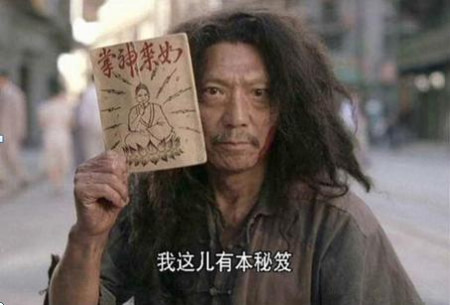
\includegraphics[width=\textwidth]{../figs/secret_kungfu.jpg}
  \end{center}
\end{frame}

\begin{frame}
  \frametitle{But this talk is really about...}
  \begin{center}
    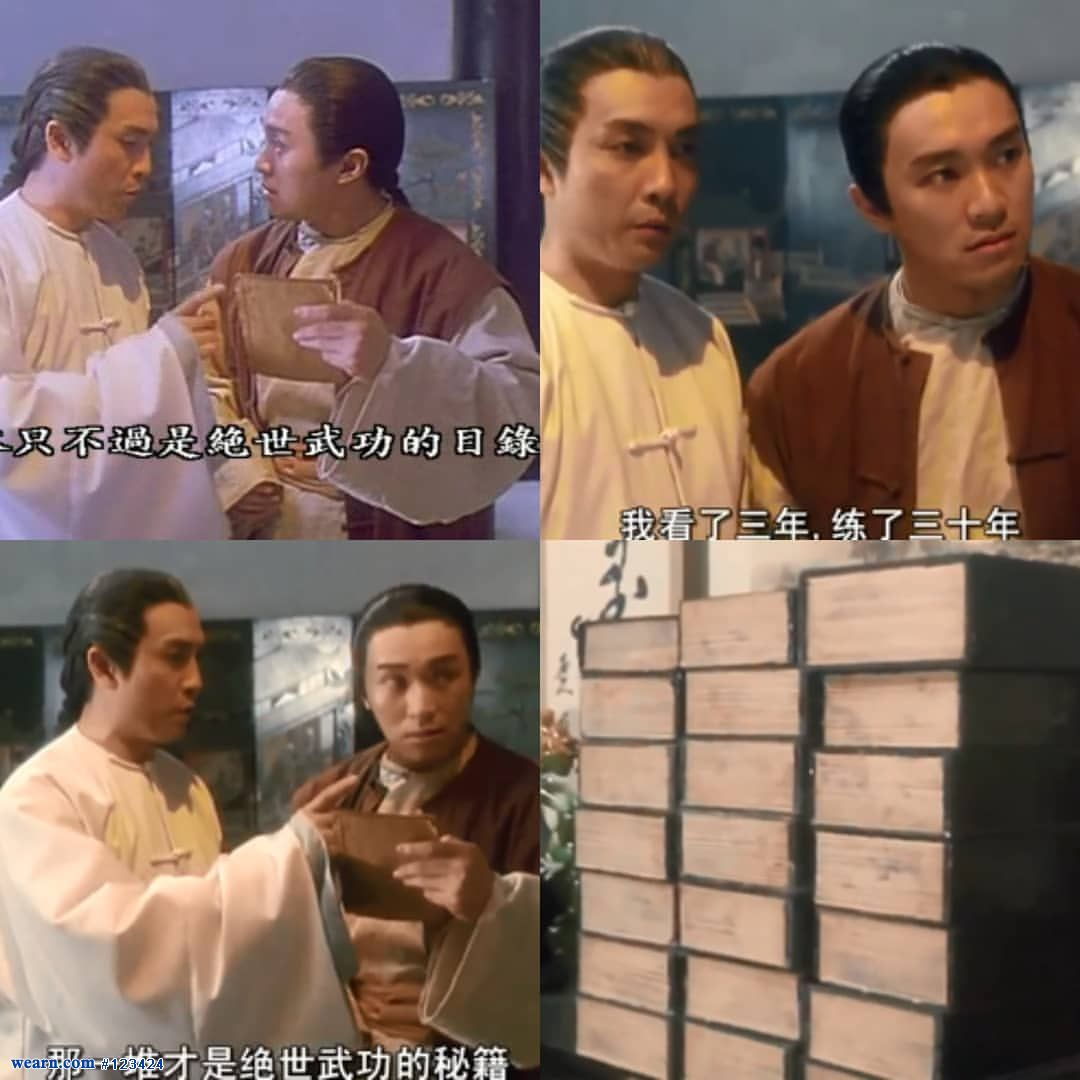
\includegraphics[height=0.8\textheight]{../figs/kungfu_category.jpg}
  \end{center}
\end{frame}

\section*{Outline}
\frame{\tableofcontents}

\section{Base Facts}

\begin{frame}
  \frametitle{The Recent Rise of Databases}
  \begin{columns}
    \begin{column}{0.4\textwidth}
      \begin{block}{Big Data}
        \begin{itemize}
          \item large volumn
          \item low value per MB
        \end{itemize}
      \end{block}
      \begin{block}{New Infrastructures}
        \begin{itemize}
          \item storage
            \begin{itemize}
              \item speed: PCIE, SSD, eNVM
              \item cost: high-volumn disk
            \end{itemize}
          \item network: 10G, 25G
          \item software: DIO/AIO, dpdk/spdk
        \end{itemize}
      \end{block}
    \end{column}
    \begin{column}{10px}
      \Large \textcolor{blue}{$\Rightarrow$}
    \end{column}
    \begin{column}{0.45\textwidth}
      \begin{exampleblock}{The Recent Rise of Databases}
        \begin{itemize}
          \item more scenarios
            \begin{itemize}
              \item in-memory
              \item embedded
              \item queue
              \item many available zones
            \end{itemize}
          \item more data models
            \begin{itemize}
              \item relational
              \item key-value
              \item spatial
              \item document
              \item time-series
              \item graph
            \end{itemize}
        \end{itemize}
      \end{exampleblock}
    \end{column}
  \end{columns}
  \note[item]{
    Large volumn data push high TPS databases:
    \begin{enumerate}
      \item adoption of LSM and other trees, rather than typical B/B+ trees.
      \item software-defined network, in order to reduce in-IDC impactness between storage clusters and other businesses.
    \end{enumerate}
  }
  \note[item]{
    Low value per MB incubates:
    \begin{enumerate}
      \item adoption of eventual consistency
      \item batch\&streaming computation engines
      \item anti-normal form table designs
    \end{enumerate}
  }
\end{frame}

\begin{frame}
  \frametitle{Basic Facts}
  \begin{quotation}
    Sequential access to disk, be it magnetic or SSD, to be at least three orders of magnitude faster than random IO.
  \end{quotation}
\end{frame}

\section{Message Queues}
\frame{\tableofcontents[currentsection]}

\begin{frame}
  \frametitle{OpLog}

  \begin{block}{Scenarios}
    Despite of slight differences,
    \emph{operation log} (a.k.a., \emph{op-log}) is also known as
    \emph{journal}, \emph{commit log}, \emph{write-ahead log (WAL)},
    \emph{redo log} and \emph{replication log}.
    As these names indicate, it is suitable for
    \begin{itemize}
      \item in-memory state rebuilding (on database fail-over)
      \item database replication
      \item message queues
    \end{itemize}
    So, which pattern of read/write is required?
  \end{block}
  \begin{exampleblock}<2>{Answer}
    \begin{itemize}
      \item write in sequence
      \item randomly seek (with opaque addresses), then read sequentially from that point
      \item usually of a limited time-to-live (TTL)
    \end{itemize}
  \end{exampleblock}
  \note[item]<2>{
    Most modern filesystems, e.g., ext4, are also journalized.
    A possible optimization for a journalized db is to disable fs's journal.
  }
\end{frame}

\begin{frame}
  \frametitle{OpLog: logical structure}
  \begin{center}
    \includegraphics{../figs/oplog.pdf}
  \end{center}
  \begin{block}{~}
    \begin{itemize}
      \item An OpLog is logically an infinite sequence of operations (put, modify, delete).
      \item Then, how to implement inifinite sequences which can be \emph{seeked}, \emph{scanned} and \emph{truncated}?
    \end{itemize}
  \end{block}
\end{frame}

\begin{frame}[t]
  \frametitle{OpLog: physical structure}
  \begin{center}
    \includegraphics{../figs/oplog_in_practice.pdf}
  \end{center}
  \begin{block}{Epoch}
    OpLog is splitted into multiple segments.
    Each is called an \emph{epoch}.
    \begin{itemize}
      \item So once fail-over, one must not open any epoch file to make SN strictly increasing.
      \item TTL is simply removing outdated epoch files.
    \end{itemize}
  \end{block}
\end{frame}

\begin{frame}
  \frametitle{OpLog: Q\&A}
  \begin{block}{~}
    \begin{itemize}
      \item Q: How to avoid write amplification?
      \item<2-> A: Batching
        \begin{itemize}
          \item an interesting question: what means a write is ``OK''?
        \end{itemize}
      \item Q: What are disadvantages of oplog?
      \item<3> A: Two
        \begin{enumerate}
          \item information density
          \item query efficiency
        \end{enumerate}
    \end{itemize}
  \end{block}
  \note[item]<2>{
    Notes for ``OK writes''.
    Answers to this question lead to different products.
    For example,
    \begin{itemize}
      \item Zookeeper honors on-disk.
      \item Redis chooses in-memory.
      \item Kafka gives choices to users.
    \end{itemize}
    While considering distributed replicas, answers will be more complicated.
  }
  \note[item]<3>{
    Notes for ``query efficiency''.
    OpLog is natually time-windowed.
    But most queries to a typical database is not related to time.
  }
\end{frame}

\section{Key-Value Storage}
\frame{\tableofcontents[currentsection]}

\subsection*{B+ Tree}

\begin{frame}[t]
  \frametitle{B+ Tree}
  \begin{center}
    \includegraphics{../figs/b_plus_tree_origin.pdf}
  \end{center}
  \note[item]{
    Key properties to B+ trees:
    \begin{enumerate}
      \item values are stored outside the tree
      \item leaves are chained as a list
    \end{enumerate}
    This structure achieves excellent performance in both point query and range query.
  }
\end{frame}

\begin{frame}[t]
  \frametitle{B+ Tree}
  \begin{center}
    \includegraphics{../figs/b_plus_tree_insert3.pdf}
  \end{center}
  \note[item]{
    When add a new key-value pair $(3,v_3)$,
    one have to
    \begin{enumerate}
      \item put $v_3$ somewhere;
      \item walk through a path from the root to the appropriate leaf;
      \item insert the key 4 and point it to the location of $v_3$.
    \end{enumerate}
    So, it requires $O(\log N)$ disk accesses to insert a single key.
  }
  \note[item]{
    Single writes will cause penality of write.
    Because even a little bytes are going to write,
    disks will read the entire block back to memory and then write them out.
    SSD/flash disks even have to erase the block before writing.
  }
  \note[item]{
    Batch writes are even worse.
    They cause ``shotgun writes", which are definitely unfriendly to any caching mechanism.
  }
  \note[item]{
    What about ``count''?
    It causes more writes.
    So does ``offset''.
  }
\end{frame}

\subsection*{Log-Structured Merge Tree}

\begin{frame}
  \frametitle{LSM Tree}
  \begin{block}{A short introduction}
    \begin{enumerate}
      \item It was invented in 1996.
        Google digged it out in early 00's and released its modern variant in the ``Big Table'' paper.
      \item extremely fast write
      \item balanced read
    \end{enumerate}
  \end{block}
\end{frame}

\begin{frame}
  \frametitle{LSM Tree: Level-DB favour}
  \begin{center}
    \includegraphics{../figs/lsm.pdf}
  \end{center}
  \note[item]{
    In writing,
    \begin{enumerate}
      \item A write first goes to oplog, and then, the active memtable.
      \item When the active memtable is full, it is shadowed and a new active memtable swaps in.
      \item The shadowed memtable dumps to disk and forms a $L_0$ file.
        \begin{itemize}
          \item SSTables (tables in disk) are generally B-Trees or variants, and most importantly, \emph{immutable}.
          \item $L_0$ files can be overlapped.
        \end{itemize}
      \item A background routine periodically compacts $L_i$ disk files into $L_{i+1}$.
        \begin{itemize}
          \item $L_i$ files will never be overlapped for every $i\geqslant 1$.
        \end{itemize}
    \end{enumerate}
  }
\end{frame}

\note[itemize]{
  \item In point query about key $k$,
    \begin{enumerate}
      \item Finds out all files containing $k$.
      \item Seeks $k$ in these files.
      \item Merges the results in time order.
    \end{enumerate}
    It requires $O(1)$ membership testing to achieve $O(\log N)$ IO's.
  \item What about ``count''?
    \\
    It must go through the range to get the precise number.
    (For an imprecise one, there is a fast algorithm named by HyperLogLog).
}

\begin{frame}
  \frametitle{Bloom Filter: $O(1)$ approximate membership testing}
  \begin{center}
    \includegraphics{../figs/bloomfilter.pdf}
  \end{center}
  \begin{block}{~}
    Given a fixed-size bitmap and 3 hash functions $h_0$, $h_1$ and $h_2$.
    \begin{itemize}
      \item On write, sets all $h_i(k)$.
      \item On test, tests if all $h_i(k)$ is set.
    \end{itemize}
    \emph{When it denies, there is definitely no such a key};
    but it is not true otherwise.
  \end{block}
  \note[item]{
    Google chrome engages bloomfilter to filter malicious websites.
  }
  \note[item]{
    There are some academic efforts in this area, such as cuckoo-filter.
  }
\end{frame}

\begin{frame}
  \frametitle{Skip List: An Easy Map Implementation}
  \begin{center}
    \only<1>{\includegraphics{../figs/skiplist.pdf}}
    \only<2>{\includegraphics{../figs/skiplist_seek.pdf}}
  \end{center}
  \begin{block}{~}
    \begin{itemize}
      \item A level-$n$ node has $n$ successors,
        where the level-$i$ chain links all level-$n$ nodes together for all $n\geqslant i$.
      \item The \# of level-$n$ nodes is half of \# of level-$(n-1)$ nodes.
        \begin{itemize}
          \item An incoming node is usually associated with a randomized level.
        \end{itemize}
    \end{itemize}
  \end{block}
  \note[item]<2>{
    Take $8$ for an example:
    \begin{enumerate}
      \item On the highest level (level-4), $1<8<9$.
        Then, go down alongside $1$.
      \item On level-3, $5<8<9$.
        Then, go down alongside $5$.
      \item On level-2, $7<8<9$.
        Then, go down alongside $7$.
      \item On level-1, hit $8$.
    \end{enumerate}
  }
  \note[item]<2>{
    Skip lists can easily support concurrent inserts.
    But it is not quite friendly to cache.
  }
\end{frame}

\section{Documents and Secondary Indices}
\frame{\tableofcontents[currentsection]}

\begin{frame}[fragile]
  \frametitle{Document Queries}
  \begin{center}
    \begin{minted}[autogobble]{json}
      {"name": "Alice", "age": 18}
      {"name": "Alice", "age": 20}
      {"name": "Alice", "age": 21}
      {"name": "Alan", "age": 21}
      {"name": "Alan", "age": 18}
    \end{minted}
  \end{center}
  \begin{block}{~}
    \begin{minted}[autogobble]{js}
      db.find({"name": {"$eq": "Alice"},
               "age": {"$eq": 18}})
    \end{minted}
    \begin{itemize}
      \item Queries usually condition on a small piece of fields.
      \item Results must be a set of docs.
    \end{itemize}
  \end{block}
\end{frame}

\begin{frame}
  \frametitle{Secondary Indices: A Straightforward Way}
  \begin{columns}[t]
    \begin{column}{0.5\textwidth}
      \begin{center}
        Primary Storage
        \\
        \scriptsize
        \begin{tabu}{ccl}
          DocID&&Value\\
          \hline
          0&$\rightarrow$&\{"name":"Alice","age":18\}\\
          1&$\rightarrow$&\{"name":"Alice","age":20\}\\
          2&$\rightarrow$&\{"name":"Alice","age":21\}\\
          3&$\rightarrow$&\{"name":"Alan","age":21\}\\
          4&$\rightarrow$&\{"name":"Alan","age":18\}\\
        \end{tabu}
      \end{center}
    \end{column}
    \begin{column}{0.5\textwidth}
      \begin{center}
        Secondary Indices
        \\
        \scriptsize
        \begin{tabu}{cc}
          \begin{tabu}{cc}
            name&DocID\\
            \hline
            Alan&3\\
            Alan&4\\
            Alice&0\\
            Alice&2\\
            Alice&1\\
          \end{tabu}
          &
          \begin{tabu}{cc}
            age&DocID\\
            \hline
            18&0\\
            18&4\\
            20&1\\
            21&3\\
            21&2\\
          \end{tabu}
        \end{tabu}
      \end{center}
    \end{column}
  \end{columns}
  \begin{block}{Index}
    Each is a shadowed B+ Tree.
  \end{block}
  \begin{block}{Query}
    \begin{enumerate}
      \item Selects an index
      \item Goes through such index with constraints and gets primary keys.
      \item Goes through docs by these primary keys and filters them with the whole condition one by one.
    \end{enumerate}
  \end{block}
  \note[item]{
    Cost-based optimizer (CBO): picks a small piece of docs to see which index is the most efficient over the samples.
  }
  \note[item]{
    In the straightforward way, primary keys in secondary indices are not necessarily sorted.
  }
\end{frame}

\subsection*{Lucene}

\begin{frame}[fragile]
  \frametitle{Secondary Indices: The Lucene Way}
  \begin{columns}[t]
    \begin{column}{0.4\textwidth}
      \begin{center}
        Primary Storage
        \\
        \scriptsize
        \begin{tabu}{cl}
          DocID&Doc\\
          \hline
          0&\{"name":"Alice","age":18\}\\
          1&\{"name":"Alice","age":20\}\\
          2&\{"name":"Alice","age":21\}\\
          3&\{"name":"Alan","age":21\}\\
          4&\{"name":"Alan","age":18\}\\
        \end{tabu}
      \end{center}
    \end{column}
    \begin{column}{0.55\textwidth}
      \begin{center}
        Lucene Indices
        \\
        \scriptsize
        \begin{tabu}{cc}
          \begin{tabu}{ll}
            age&DocIDs\\
            \hline
            18&0,4\\
            20&1\\
            21&2,3\\
          \end{tabu}
          &
          \begin{tabu}{ll}
            name&DocIDs\\
            \hline
            Alan&3,4\\
            Alice&0,1,2\\
          \end{tabu}
        \end{tabu}
      \end{center}
    \end{column}
  \end{columns}
  \begin{block}{Index intersection}
    \begin{minted}[autogobble]{js}
      db.find({"name": {"$eq": "Alice"}, "age": {"$eq": 21}})
    \end{minted}
    \begin{enumerate}
      \item Each atom condition forms a seekable inverted chain
        \begin{itemize}
          \item \mintinline{json}|{"name": {"$eq": "Alice"}}| forms [0,1,2].
          \item \mintinline{json}|{"age": {"$eq": 18}}| forms [0,4].
        \end{itemize}
      \item Merges these chains
        \begin{itemize}
          \item For ``or'', just external merge sort.
          \item For ``and'',
            when chain A pops a DocID which is larger than the current in chain B,
            chain B shall seek that DocID instead of popping.
        \end{itemize}
    \end{enumerate}
  \end{block}
\end{frame}

\begin{frame}
  \frametitle{Trie: A Compact Way To Index Strings}
  \begin{center}
    \includegraphics{../figs/trie.pdf}
  \end{center}
  \begin{block}{~}
    \begin{itemize}
      \item String keys are stored as a trie tree.
      \item DocIDs are formed as a skip-list to seek efficiently.
    \end{itemize}
  \end{block}
  \note[item]{
    LevelDB deploys prefix encoding instead of trie tree.
  }
\end{frame}

\begin{frame}
  \frametitle{BKD Tree}
  \begin{center}
    \includegraphics{../figs/bkd.pdf}
  \end{center}
  \begin{block}{~}
    BKD Tree is a variant of k-Dimensional Tree.
    It can be applied to
    \begin{itemize}
      \item reduce \# of opened doc chains;
      \item support spatial queries.
    \end{itemize}
  \end{block}
\end{frame}

\section{Columnar Storage and MPP Databases}
\frame{\tableofcontents[currentsection]}

\begin{frame}
  \frametitle{MPP Databases}
  \begin{block}{~}
    Another way to speed queries up is, Massively Parallel Processing.
    \emph{Columnar storage is a file format optimized for MPP.}
  \end{block}
  \note[item]{
    The key disadvantage to table-and-indices architecture is:
    \emph{duplication of data},
    which implies
    \begin{itemize}
      \item large storage cost,
      \item weak consistency, or complicated transaction implementation.
    \end{itemize}
  }
\end{frame}

\begin{frame}
  \frametitle{Columnar Storage}
  \begin{center}
    \includegraphics{../figs/columnar.pdf}
  \end{center}
  \begin{block}{Advantages}
    \begin{itemize}
      \item high compression
      \item queries only read related columns
    \end{itemize}
  \end{block}
\end{frame}

\section{Spatial Databases}
\frame{\tableofcontents[currentsection]}

\begin{frame}
  \frametitle{Spatial Databases}
  \begin{block}{~}
    Spatial databases must answer spatial questions such as
    \begin{itemize}
      \item Which records are located in a given area?
      \item Which record is the nearest to a given point?
    \end{itemize}
  \end{block}
\end{frame}

\note[enumerate]{
  \item LBS incubates modern, large-scale, spatial databases.
}

\begin{frame}
  \frametitle{R-Tree}
  \begin{columns}[t]
    \begin{column}{0.3\textwidth}
      ~\\
      \includegraphics{../figs/rtree_planar.pdf}
    \end{column}
    \begin{column}{0.4\textwidth}
      ~\\
      \includegraphics{../figs/rtree.pdf}
    \end{column}
  \end{columns}
  \begin{block}{~}
    Each (sub-)tree has a bounding box.
    And, queries shall be translated to something about a bounding box.
    \begin{itemize}
      \item ``locate in an area'': does a bounding box overlap the area?
    \end{itemize}
  \end{block}
  \note[item]{
    There are a lot of variants, e.g., R+ tree, R* tree, QR tree and KD tree.
    A key difference is, ``can bounding boxes overlap?''
    And thus, they will perform significantly different on highly dimensional data.
  }
\end{frame}

\begin{frame}
  \frametitle{Geo-Hash}
  \begin{columns}[t]
    \begin{column}{0.4\textwidth}
      ~\\
      \includegraphics{../figs/geohash.pdf}
    \end{column}
    \begin{column}{0.4\textwidth}
      ~\\
      \includegraphics{../figs/geohash_grids.pdf}
    \end{column}
  \end{columns}
  \begin{block}{~}
    It encodes a coordinate:
    \begin{enumerate}
      \item turns both latitude and longitude to numbers between [0, 1) (in binary);
      \item picks bits interleavingly.
    \end{enumerate}
    When one more bit is considered, the area decreases halfly.
    So, \emph{spatial questions can be translated to range queries with fixed prefix.}
  \end{block}
\end{frame}

\section{Time-Series Databases}
\frame{\tableofcontents[currentsection]}

\begin{frame}
  \frametitle{Time-Series Databases}
  \begin{block}{Features of Time-Series Queries}
    \begin{itemize}
      \item Each record is associated with a time point.
      \item Usually of very large volume. But very few updates.
      \item Records are usually recycled by Time-To-Live (TTL).
      \item Queries are usually limited in a time window.
      \item The later, the more valuable, and thus usually hotter.
      \item Query pattern may probably change over time.
    \end{itemize}
  \end{block}
\end{frame}

\begin{frame}
  \frametitle{Time-Series Databases}
  \begin{block}{~}
    Special optimizations in both write side and read side are required.
    \emph{General purpose databases are not suitable.}
    \begin{itemize}
      \item write: extremely high throughput
        \begin{itemize}
          \item<2> write-optimized structure, e.g., LSM
          \item<2> For TTL: time-window based compaction
          \item<2> For value decay: compaction on old files engages high-ratio compression
        \end{itemize}
      \item read: free schema support is necessary
        \begin{itemize}
          \item<2> Lucene style index, or columnar storage
        \end{itemize}
      \item consistency: basically eventual consistency is good enough
        \begin{itemize}
          \item<2> WAL is not necessary
        \end{itemize}
    \end{itemize}
  \end{block}
\end{frame}

\section*{References}
\frame{\tableofcontents}

\begin{frame}
  \frametitle{References}
  \begin{itemize}
    \item \url{http://www.benstopford.com/2015/02/14/log-structured-merge-trees/}
    \item \textsl{The Log-Structured Merge-Tree} by O'Neil, et al.
    \item \url{https://zhuanlan.zhihu.com/p/35814539}
  \end{itemize}
\end{frame}

\end{document}
